\chapter{Konzept und Implementierung}\label{chap:concept}

\section{Konzept}\label{sec:concept}

Das Programmablauf wird in einzelne Schritte unterteilt, auf die in den nächsten Kapiteln näher eingegangen werden.
\\\\
\begin{figure}[ht]
  \centering
  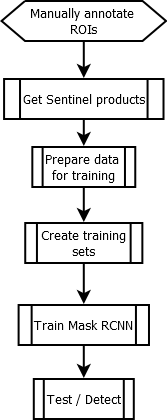
\includegraphics[width=.2\textwidth]{pics/overview.PNG}
  \caption{Gesamtablauf der Anwendung}
  \label{fig:overview}
\end{figure}
Zuerst müssen die Daten für das Training bzw. für die Erkennung manuell annotiert werden. Diese Metadaten werden dann genutzt, um automatisch Sentinelprodukte\footnote{Aufnahmenpakete der Sentinel-Plattformen werden als Produkte bezeichnet.} mittels einer API\footnote{Copernicus Open Access Hub \url{https://scihub.copernicus.eu/}}, die von der Copernicus zur Verfügung gestellt wird, herunterzuladen. Aus den Produkten werden die relevanten Bänder extrahiert und unter anderem die jeweiligen NDVI-Werte berechnet. Nachdem die Produkte für das Training vorbereitet wurden, werden die Daten in ein Trainings- und in ein Validierungsdatensatz aufgeteilt. Der folgende Trainingsprozess basiert auf diesen Datensätzen. Sobald das Training abgeschlossen ist, kann die Performanz des Modells getestet werden. 

\section{Annotation}\label{sec:annotation}

Zu Beginn werden die Regionen, die entweder für das Training benutzt oder überprüft werden, per Hand definiert. Vorrausgesetzte Informationen sind
\begin{itemize}
	\item Geografische Koordinaten,
	\item Zeitraum des Befalls und
	\item Bezeichnung der Infektion.
\end{itemize}
Als Format dieser Informationen dient \textit{GeoJSON}\footnote{GeoJSON ist eine Erweiterung des JSON-Format und beschreibt geografische Daten und Geometrien. GeoJSON wird durch den RFC7946-Standard definiert.}. GeoJSON enthält nicht nur geografische Daten, sondern ist auch um benutzerdefinierte Metadaten erweiterbar.

\begin{lstlisting}[language=json,caption={Beispiel einer Annotation},captionpos=b]
{
  "type": "Feature",
  "properties": {
    "disease": 1,
    "incubation": "14DAYS",
    "date": "2018-07-19T13:00:00Z"
  },
  "geometry": {
    "type": "Polygon",
    "coordinates": [
      [
        [11.171988617177981, 44.574291380353003],
        [11.1726616444942, 44.574017992242283],
        ...
      ]
    ]
  }
}
\end{lstlisting}
